\documentclass{report}
\usepackage{graphicx}
\usepackage[utf8]{inputenc}
\usepackage[T1]{fontenc}
\usepackage{pgfplots}
\usepackage{pgfplotstable} 
\usepackage{titlesec}
\usepackage{lipsum}
\usepackage{authblk}
\usepackage{algorithm}
\usepackage[noend]{algpseudocode}
\usepackage {tikz}
\usetikzlibrary {positioning}

\titleformat{\chapter}[display]{\normalfont\bfseries}{}{0pt}{\Large}

\begin{document}

\title{Projeto e Análise de Algoritmos: Trabalho Prático 1}
\author{João Mateus de Freitas Veneroso}
\affil{Departamento de Ciência da Computação da Universidade Federal de Minas Gerais}

\maketitle

\tableofcontents

\chapter{Introdução}

Este relatório descreve a implementação do trabalho prático 1 da disciplina Projeto e Análise de Algoritmos. 
O trabalho consistiu em modelar um aplicativo de compartilhamento de viagens por meio do uso de grafos. A 
descrição mais detalhada do problema e do algoritmo utilizado para resolvê-lo será feita na próxima seção.

\chapter{Implementação}

\section{Problema} 

Sendo $ G = (V, A) $ um grafo onde os vértices $ v \in V $ representam rotas e as arestas direcionadas $ (v_i, v_j) \in A $ representam
possibilidades de compartilhamento, cada aresta possui um benefício associado $ B(v_i, v_j) \in R^* $ e cada rota possui uma capacidade
igual ao número de assentos vazios no veículo.
Um plano de compartilhamento é um subgrafo
$ G_p = (V, A_p) : A_p \subseteq A $ que contém todos os vértices e um subconjunto das arestas de $ G $. O somatório dos benefícios
de todas as arestas representa o benefício total de um plano de compartilhamento $ B_t(G_p) = \sum_{(v_i, v_j) \in A_p} B(v_i, v_j) $.
Nosso objetivo é encontrar um plano de compartilhamento $ G_p^* = argmax $ $ B_t(G_p) $ sujeito às restrições:

\begin{itemize}
\item O número total de passageiros em um veículo não pode exceder a sua capacidade.
\item Um passageiro só pode pegar carona em uma rota. Ou seja, $\forall (v_i, v_j) \in A_p $ não existe $ k \neq j $ tal que $ (v_i, v_k) \in A_p $.
\item Um motorista não pode ser também passageiro e vice-versa. Ou seja, $\forall (v_i, v_j) \in A_p $ não existe $ k $ tal que $ (v_j, v_k) \in A_p $.
\end{itemize}

\section{Solução} 

O plano de compartilhamento de benefício máximo $ G_p^* $ é um subgrafo de $ G $ em que todos os vértices são mantidos, mas cujas
arestas são um subconjunto das arestas de $ G $. Dessa forma, uma solução para o problema é construir todas as combinações possíveis 
$ G_p $, conferir sua validez de acordo com as restrições descritas na subseção anterior e finalmente calcular o benefício total. 
Após calcularem-se todas as configurações possíveis, escolhe-se aquela com o maior benefício dentre as possibilidades e assim obtemos $ G_p^* $. 

O algoritmo \ref{alg:alg_1} descreve esta abordagem. Primeiro inicializa-se o benefício máximo $ b^* $ com um valor negativo, dessa
forma qualquer configuração válida vai proporcionar um benefício maior. A partir daí, no loop das linhas 5-10, para cada configuração
válida, calcula-se o benefício total e atualiza-se o valor de $ b^* $ se este benefício for maior do que qualquer um encontrado até então.
Além disso, a variável $ G_p^* $ guarda a configuração que proporcionou o maior benefício. Ao final do algoritmo, $ b^* $ guarda o valor 
do benefício máximo para o grafo $ G $ e $ G_p^* $ guarda a configuração que proporcionou este benefício. 

A complexidade deste algoritmo depende do número de configurações $ G_p $ diferentes e do custo da função $ ConstraintsAreValid $. O número de 
configurações $ G_p $ diferentes é $ 2^m $ para $ m $ igual ao número de arestas no grafo $ G $. Pois, cada aresta pode estar presente ou
não em $ G_p $ e nós queremos as combinações possíveis para todas as arestas m. O custo da função $ ConstraintsAreValid $ depende do número de 
arestas, pois, para cada aresta $ (u,v) $, temos de verificar se ela é a única aresta que sai do vértice $ u $, se o vértice $ v $ é um motorista
e se $ v $ possui espaço para acomodar todos os passageiros de $ u $. Como todas estas operações tem custo constante, a função $ ConstraintsAreValid $ 
tem custo $ O(m) $. Por último, a linha 7 calcula a soma dos pesos de todas as arestas também com custo $ O(m) $. Logo, 
a complexidade total do algoritmo é $ 2m2^m $ e o algoritmo é $ O(m2^m) $.

\begin{algorithm}
\caption{MaximizeBenefit}\label{euclid}
\begin{algorithmic}[1]
\Procedure{MaximizeBenefit}{G = (V,A)}

\State $ b^* \gets -1 $
\State $ G_p^* \gets \emptyset $
\item \ForAll{\textit{$ G_p = (V, A_p) : A_p \subseteq G.A $}}

\If {\textit{ConstraintsAreValid($G_p$)}}
  \State $ \textit{b} \gets \sum_{(v_i, v_j) \in A_p} B(v_i, v_j) $
  \If {$ b > b^* $}
    \State $ b^* \gets b $
    \State $ G_p^* \gets G_p $
  \EndIf
\EndIf
\EndProcedure
\end{algorithmic}
\label{alg:alg_1}
\end{algorithm}

\definecolor {processblue}{cmyk}{0.96,0,0,0}
\begin{figure}
\begin {center}
\begin {tikzpicture}[-latex ,auto ,node distance =4 cm and 5cm ,on grid ,
semithick ,
state/.style ={ circle ,top color =white , bottom color = processblue!20 ,
draw,processblue , text=blue , minimum width =1 cm}]
\node[state] (Z) {$Z$};
\node[state] (X) [above left=of Z] {$X$};
\node[state] (Y) [above right =of Z] {$Y$};
\path (X) edge node[below =0.15 cm] {$5$} (Z);
\path (X) edge node[above] {$10$} (Y);
\end{tikzpicture}
\end{center}
\caption{Grafo 1} 
\label{fig:graph}
\end{figure}

Uma melhora ainda pode ser alcançada se deixarmos de testar parte das configurações inválidas de $ G $. Sabemos que 
um passageiro só pode pegar carona em uma rota, portanto, qualquer combinação $ G_p $ onde existirem arestas $ (u, v_i), (u, v_j) : i \neq j $
é inválida. Dessa forma, basta manter uma única aresta ativa por vez na lista de adjacência de cada vértice. Por exemplo, na figura \ref{fig:graph} apenas 
duas combinações precisam ser testadas: $ G_0(V,A_0) : A_0 = \{(X,Y)\} $ e $ G_1(V,A_1) : A_1 = \{(X,Z)\} $.

Além disso, é necessário lembrar que um vértice pode representar um motorista sem passageiros ou um passageiro que não vai pegar carona com ninguém, 
portanto, o número total de combinações 
se torna $ \sum_{v \in V} G \rightarrow Adj(v) + 2 $ e, no pior caso (um grafo completo), o número de combinações se torna $ O(n^n) $ 
onde n é o número de vértices no grafo $ G $. Feitas estas considerações, a complexidade assintótica do algoritmo é $ O(mn^n) $.
O algoritmo implementado em Python para este trabalho utiliza este método.

A complexidade de espaço do algoritmo original e da versão aprimorada é $ O(n + m) $, pois o grafo é armazenado na forma de listas de adjacência.

\chapter{Experimentos}

\begin{figure}
  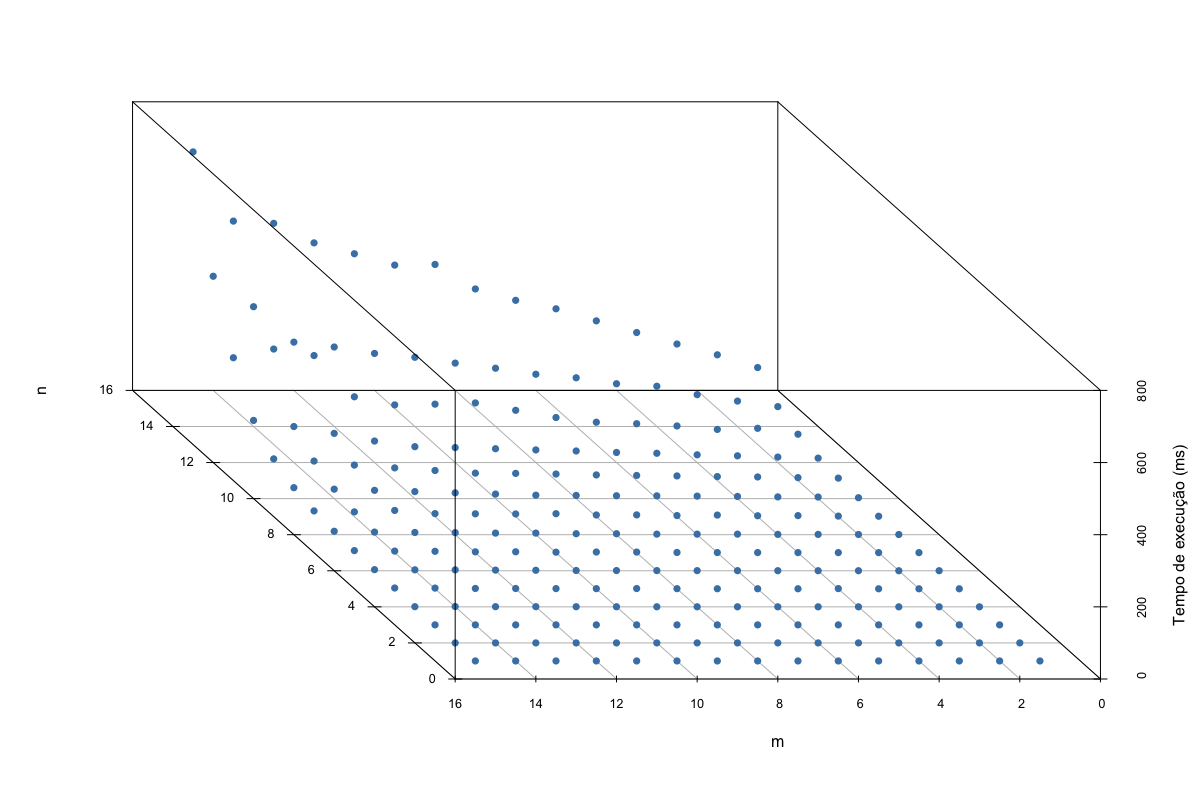
\includegraphics[width=\linewidth]{execution_time.png}
  \caption{Tempo de execução variando n e m}
  \label{fig:execution_time}
\end{figure}

\begin{figure}
  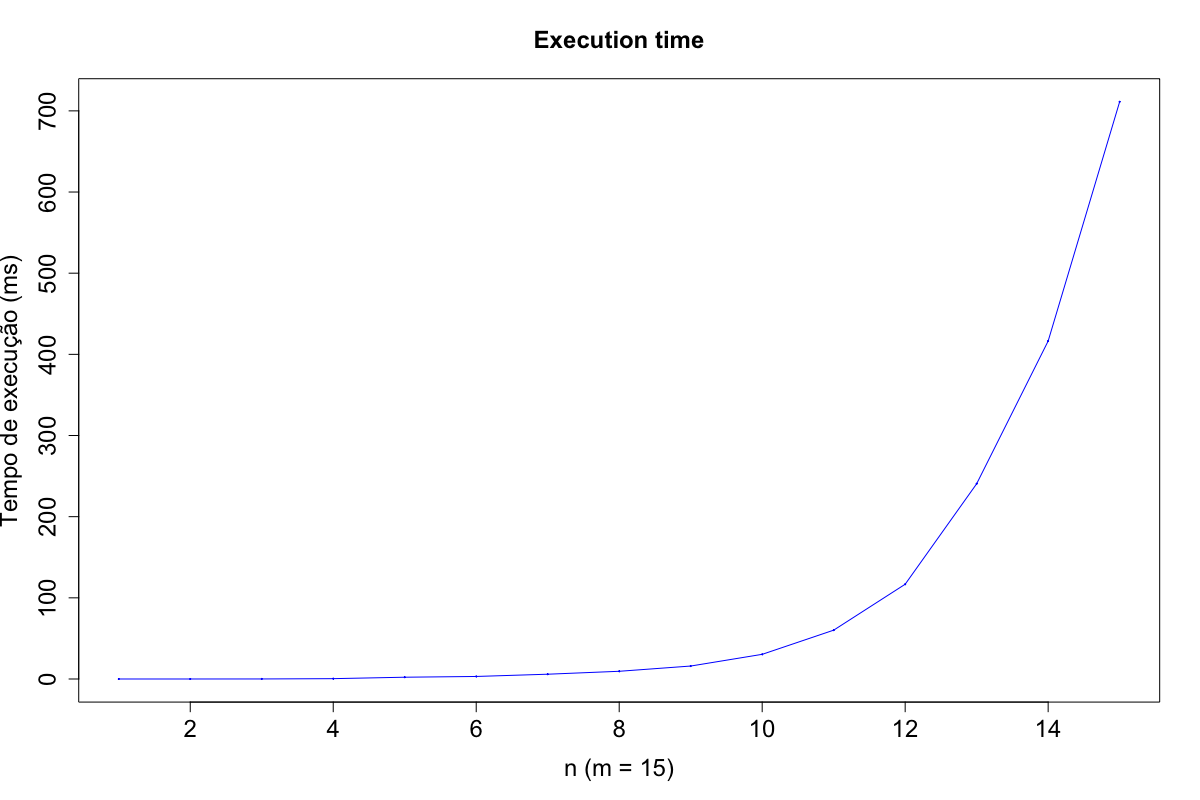
\includegraphics[width=\linewidth]{n.png}
  \caption{Tempo de execução variando n}
  \label{fig:n}
\end{figure}

\begin{figure}
  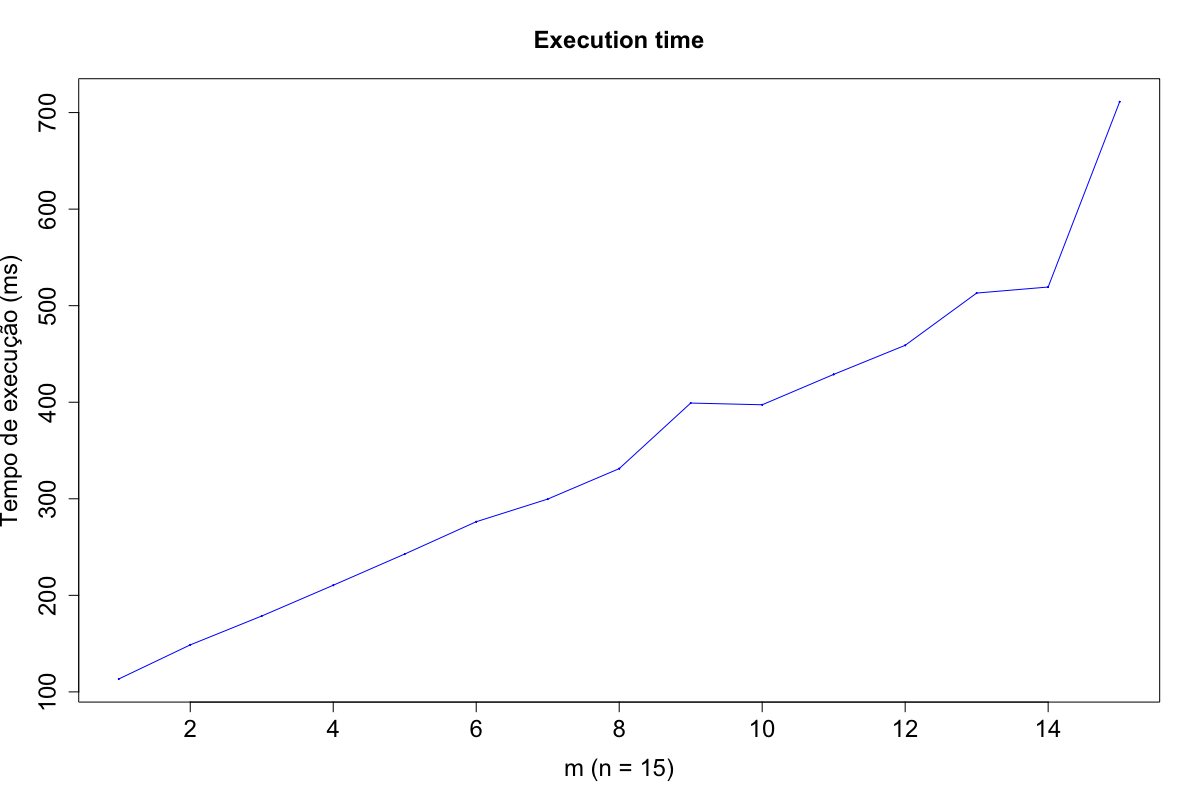
\includegraphics[width=\linewidth]{m.png}
  \caption{Tempo de execução variando m}
  \label{fig:m}
\end{figure}

Um experimento foi conduzido para verificar a complexidade assintótica do algoritmo descrito na última seção. Para tanto,
foram gerados grafos aleatórios com a quantidade de vértices variando entre 1 e 15 e a quantidade de arestas variando
também entre 1 e 15. Observe que, por exemplo, um grafo com dois vértices pode ter no máximo duas arestas, nesses casos, 
o número de arestas descrito nos experimentos serve como um limite superior para o número de arestas total do grafo. O
gráfico \ref{fig:execution_time} mostra como o tempo de execução (mensurado em milisegundos) variou com mudanças tanto no número de arestas m como
no número de vértices n. É possível observar que a medida que os valores de m e n crescem, o tempo de execução cresce de forma exponencial.
O gráfico \ref{fig:n} é um corte do gráfico tridimensional que mantém m fixo com o valor de 15 arestas e varia n. O gráfico \ref{fig:m} é um corte
do gráfico tridimensional que varia m e mantém o valor de n fixo em 15 vértices. 
É possível observar nestes cortes que a complexidade cresce de forma semilinear em m e claramente exponencial em n, como
previsto pela função de complexidade assintótica. 

\chapter{Conclusão}

Este relatório descreveu a implementação do Trabalho Prático 1 da disciplina Projeto e Análise de Algoritmos. A complexidade
final alcançada foi $ O(mn^n) $ e os resultados experimentais se mostraram coerentes com as expectativas teóricas.

\end{document}
